%Chapter 2
\chapter*{Exemplos de tabela e figura}
\addcontentsline{toc}{chapter}{Exemplos de tabela e figura}
\fancyhead[RO]{\slshape Exemplos de tabela e figura}  % Mark on right odd pages
\fancyhead[LE]{\slshape Deutschkurs}     % Mark on left even pages

 Figura pós-formata\c{c}\~ao:
\begin{figure}[H]
    \centering
    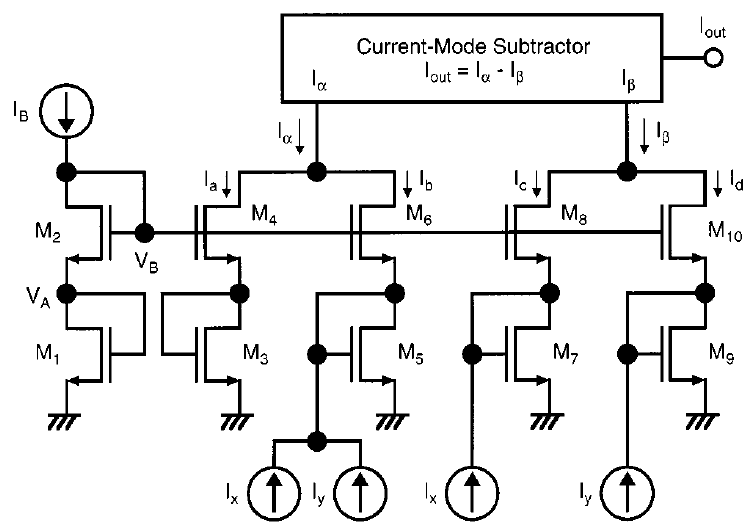
\includegraphics[width=0.5\textwidth]{figures/tanno_multiplier.png}
    \caption{\small Multiplicador de quatro quadrantes proposto em \cite{einstein1905}.\normalsize}
    \label{fig_tanno}
\end{figure}

Tabela simples:
\begin{table}[h]
    \centering
    \caption{Razões de aspecto}
    \label{tab_aspectos}
    \begin{tabular}{|l|r|r|}
    \hline
    Transistor                    & W/L ($\mu$m/$\mu$m) \\ \hline
    M$_1$ e M$_2$                 & 10/0,5              \\ \hline
    M$_3$ a M$_{10}$              & 3,5/0,5             \\ \hline
    M$_{11}$ a M$_{18}$           & 40/0,5              \\ \hline
    M$_{19}$ a M$_{22}$           & 3,5/0,5             \\ \hline
    M$_{1N}$ a M$_{4N}$           & 2,0/0,5             \\ \hline
    M$_{1P}$ a M$_{6P}$           & 20/0,5              \\ \hline
    \end{tabular}
\end{table}

\lipsum[1-25]